
\documentclass{exam}
\usepackage{tikz}

\begin{document}
\printanswers

\section{Domande Teoria}

\begin{questions}
    \question Esprimere la condizione necessaria e sufficiente affinché una scomposizione sia senza perdita di informazione.
    \begin{solution}
    Sia R(A) uno schema con dipendenze funzionali F, decomposto in $\{R1(A1), R2(A2)\}$ dove $A_1 \cup A_2 = A$ \\
    La decomposizione di ogni istanza corretta(*) r(A) di  R(A) è senza perdita di informazione se e solo se  (condizione necessaria e sufficiente) \\  
    $(A1\cap A2$ superchiave di $A1)\vee(A1 \cap A2 $ superchiave di $A2) $
    \end{solution}
    \question A proposito di gestione della concorrenza descrivere il protocollo di lock a due fasi (2PL) e quello di lock a due fasi stretto.
    \question Riportare la definizione di protocollo 2PL (two-phase lock) stretto
    \question Dire cos’è e quali problemi risolve il protocollo 2PL (due fasi) stretto.
    \begin{solution}
        Il $2PL$ è un protocollo in cui le transazioni acquisiscono i \textbf{lock} nel tempo, ma, una volta \textbf{rilasciato almeno un lock}, non se ne potranno più
        acquisire. Si chiama \textbf{Two-Phase} perché le due fasi sono quella di \textbf{acquisizione} e \textbf{rilascio}.
        \\
        Il $2PL$ stretto è un \textbf{protocollo a due fasi modificato}. Le differenze stanno nella seconda fase, quando si inizia il rilascio dei \textbf{lock}:
        \begin{itemize}
            \item $T_i$ acquisice \textbf{lock} finché può (sia $LS$ che $LX$)
            \item Quando inizia il rilascio può solo rilasciare i $LS$
            \item I $LX$ verranno rilasciati solo al termine (\textbf{commit} o \textbf{rollback})
        \end{itemize}
        Questa soluzione, più rigida del $2PL$, risolve il problema dei \textbf{rollback a cascata} in quanto le altre transazioni non hanno avuto accesso
        agli oggetti \textbf{modificati} da $T_i$
    \end{solution}
    \question Dire in cosa consiste la tecnica del dump/restore (ripresa a freddo) e quando si rende necessaria.
    \question Esporre la differenza tra indici densi ed indici sparsi
    \begin{solution}
        Gli \textbf{Indici Densi} sono indici con tante chiavi di ricerca quanti sono i valori distinti dell'attributo su cui sono costruiti.\\
        Gli \textbf{Indici Sparsi} sono indici in cui nelle foglie non ci sono più tutti i valori distinti della chiave di ricerca ma \textbf{solo un valore} (il \textbf{massimo}).
    \end{solution}
    \question Riportare la definizioe di chiusura di un insieme di attributi
    \begin{solution}
        La chiusura di un insieme di dipendenze funzionali $F$ è un insieme di dipendenze funzionali $F^+$ tali che ogni dipendenza funzionale $f^+$ dell'insieme $F^+$ sia derivabile da $F$ 
        \\(l'insieme $F^+$ è finito)
    \end{solution}
    \question Spiegare la differenza tra ottimizzazione logica ed ottimizzazione fisica di un'interrogazione
    \begin{solution}
        \textbf{L'ottimizzatore logico} lavora sull'albero di parsificazione\\
        \textbf{L'ottimizzatore fisico} considera l'albero prodotto dall'ottimizzazione logica e scegliere gli algoritmi da abbinare ai nodi operativi
    \end{solution}
    \question Dare la definizione di insieme di copertura minimale
    \begin{solution}
        Un insieme $F'$ di dipendenze funzionali è un insieme di  copertura minimale rispetto ad $F$ quando:
        \begin{enumerate}
            \item $F'$ è equivalente ad $F$
            \item ogni $X \rightarrow Y \in F'$ è in forma canonica, cioè $Y$ è un attributo
            \item ogni $X \rightarrow Y \in F'$ è priva di attributi estranei 
            \item ogni $X \rightarrow Y \in F'$ non è ridondante
        \end{enumerate} 
    \end{solution}
    \question Riportare la definizione di BCNF
    \begin{solution}
        \textbf{BCNF} è una \textbf{forma normale} per una relazione $r$ in cui ogni dipendenza funzionale (non banale, $A \rightarrow A$)
        $X \rightarrow A$ definita su di essa, $X$ contiene una chiave $K$ di $r$, cioè $X$ è superchiave per $r$.
        \begin{enumerate}
            \item $Y \subseteq X (X \rightarrow Y$ è \textbf{riflessiva})
            \item $X$ è \textbf{superchiave}
        \end{enumerate}
    \end{solution}
    \question Elencare e spiegare brevemente le proprietà ACID delle transazioni
    \begin{solution}
        \begin{description}
            \item[Atomicità (Gestore del Ripristino)] \hfill \\ il processo deve essere suddivisibile in un numero finito di unità indivisibili, chiamate transazioni. L'esecuzione di una transazione perciò deve essere per definizione o totale o nulla, e non sono ammesse esecuzioni parziali; un processo, anche parziale, invece, in quanto insieme di transazioni può non essere elementare.
            \item[Consistenza (Gestore delle Trasazioni e Serializzatore)] \hfill \\ il database rispetta i vincoli di integrità, sia a inizio che a fine transazione. Non devono verificarsi contraddizioni (incoerenza dei dati) tra i dati archiviati nel DB;
            \item[Isolamento (Serializzatore)] \hfill \\ ogni transazione deve essere eseguita in modo isolato e indipendente dalle altre transazioni, l'eventuale fallimento di una transazione non deve interferire con le altre transazioni in esecuzione;
            \item[Durabilità (Gestore del Buffer)] \hfill \\ detta anche persistenza, si riferisce al fatto che una volta che una transazione abbia richiesto un commit work, i cambiamenti apportati non dovranno essere più persi. Per evitare che nel lasso di tempo fra il momento in cui la base di dati si impegna a scrivere le modifiche e quello in cui li scrive effettivamente si verifichino perdite di dati dovuti a malfunzionamenti, vengono tenuti dei registri di log dove sono annotate tutte le operazioni sul DB.
          \end{description}
    \end{solution}
    \question Definire la nozione di azioni in conflitto in una storia $S$
    \begin{solution}
        Le azioni di una storia $S$ sono in conflitto quando:
        \begin{enumerate}
            \item appartengono a diverse transazioni,
            \item operano sullo stesso valore e
            \item \textbf{almeno una} delle due è una operazione di \textbf{write}
        \end{enumerate}
    \end{solution}
    \question Descrivere il problema del deadlock avvalendosi del grafo di attesa
    \begin{solution}\\
        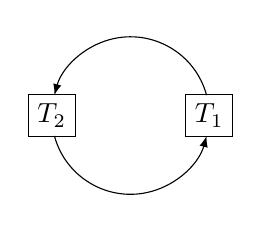
\begin{tikzpicture}

            \def \n {2}
            \def \radius {1cm}
            \def \margin {15} % margin in angles, depends on the radius
            
            \foreach \s in {1,...,\n}
            {
              \node[draw, rectangle] at ({360/\n * (\s - 1)}:\radius) {$T_{\s}$};
              \draw[->, >=latex] ({360/\n * (\s - 1)+\margin}:\radius) 
                arc ({360/\n * (\s - 1)+\margin}:{360/\n * (\s)-\margin}:\radius);
            }
            \end{tikzpicture}
            \\
            In questa situazione $T_1$ è in attesa di un rilascio da parte di $T_2$ e $T_2$ è in attesa di un rilascio da parte di $T_1$.\\
            Il grafo di attesa presenta un \textbf{ciclo}, e quando ce n'è uno ci troviamo in una situazione di deadlock.
    \end{solution}
    \question Presentare una tecnica di \textbf{superamento} del deadlock
    \begin{solution}
        \begin{itemize}
            \item Analisi del grafo di attesa (\textbf{NON Grafo dei conflitti})\\
            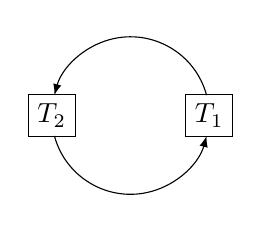
\begin{tikzpicture}

                \def \n {2}
                \def \radius {1cm}
                \def \margin {15} % margin in angles, depends on the radius
                
                \foreach \s in {1,...,\n}
                {
                  \node[draw, rectangle] at ({360/\n * (\s - 1)}:\radius) {$T_{\s}$};
                  \draw[->, >=latex] ({360/\n * (\s - 1)+\margin}:\radius) 
                    arc ({360/\n * (\s - 1)+\margin}:{360/\n * (\s)-\margin}:\radius);
                }
                \end{tikzpicture}
            \item 
                \begin{description}
                    \item[Timeout] \hfill \\ Non viene costruito nessun grafo particolare, ma viene valutato da quanto tempo una transazione è in \textbf{wait}.\\
                    Se è in wait da molto tempo (è in \textbf{timeout}), il DBMS la abortisce \textbf{SUPPONDENDO} che la transazione sia in \textbf{deadlock}. In questo modo si rompe il ciclo delle attese. 
                \end{description}
            \item 
                \begin{description}
                    \item[Timestamp] \hfill \\ Non richiede l'analisi di grafi di attesa, ma \textbf{PREVIENE} i deadlock. Questa tecnica è basata sui \textbf{timestamp} (tempo di arrivo di una transazione nel sistema). \\
                    Complessivamente in questo sistema non può mai formarsi il ciclo del grafo delle attese, perché gli archi di attesa possono andare solo da transazioni giovani verso transazioni vecchie.\\
                    Se una transazione più giovane arriva e acquisice il lock su $X$ e, successivamente, quella vecchia ha bisogno di $X$, allora il DBMS fa il \textbf{rollback} della giovane per far eseguire la vecchia.
                \end{description}
        \end{itemize}
    \end{solution}
    \question Presentare una tecnica di \textbf{prevenzione} del deadlock
    \begin{solution}
        \begin{description}
            \item[Timestamp] \hfill \\ Non richiede l'analisi di grafi di attesa, ma \textbf{PREVIENE} i deadlock. Questa tecnica è basata sui \textbf{timestamp} (tempo di arrivo di una transazione nel sistema). \\
            Complessivamente in questo sistema non può mai formarsi il ciclo del grafo delle attese, perché gli archi di attesa possono andare solo da transazioni giovani verso transazioni vecchie.\\
            Se una transazione più giovane arriva e acquisice il lock su $X$ e, successivamente, quella vecchia ha bisogno di $X$, allora il DBMS fa il \textbf{rollback} della giovane per far eseguire la vecchia.
        \end{description}
    \end{solution}
    \question Definire il concetto di dipendenza funzionale
    \begin{solution}
        Prendiamo come esempio una relazione cittadino in cui dal Codice Fiscale riesco a dedurre tutti gli altri attributi (nome, cognome, data di nascita, ecc.)\\
        CF $\rightarrow$ nome, cognome, data\_nascita.\\
        Ogni volta che vengono prese in esame tuple distinte di una relazione e le tuple coincidono sul valore del Codice Fiscale, 
        impongo al DBMS che anche tutti gli attributi caratterizzanti il cittadino coincidano.
    \end{solution}
    \question Enunciare il criterio di serializzabilità
    \begin{solution}
        Se partiamo da storie corrette (le diverse esecuzioni  seriali) e abbiamo una storia interfogliata, possiamo  concludere che la storia interfogliata è corretta se è \textbf{view-equivalente} ad una qualsiasi storia seriale.\\
        Il criterio di serializzabilità dice quindi che una storia \textbf{interfogliata} $S$ è corretta se è \textbf{view-equivalente} ad una storia seriale qualsiasi delle transazioni coinvolte da $S$ \\
        N.B.: date $n$ transazioni esistono $n!$ storie seriali
    \end{solution}
    \question Differenze tra $B-tree$ e $B^{+}-tree$ e vantaggi dei $B^{+}-tree$ rispetto ai $B-tree$ nella gestione degli indici
    \begin{solution}
        L'unica differenza sta nelle foglie che nel $B^{+}-tree$ hanno una chiave in più (che è la chiave \textbf{separatrice} che trovo risalendo l'albero). 
        Questo permette di collegare tra loro le foglie (quindi gli indici contenute in esse) e ciò permette di scandire sequenzialmente le foglie. Questo 
        velocizza di molto le \textbf{ricerche di range di valori}.
    \end{solution}
    \question Mostrare un esempio semplice (una relazione R ed un insieme di dipendenze funzionali F) per cui  l’algoritmo di normalizzazione in BCNF non può essere in grado di mantenere la località delle dipendenze. 
    \question Che cosa si intende per \textbf{tupla spuria}
    \question Chiarire il concetto di decomposizione con join con o senza perdita di informazione
    \question Enunciare la condizione necessaria e sufficiente di decomponibilità senza perdita di informazione di una relazione in due sottorelazioni
    \question Enunciare il criterio di view-serializzabilità di una storia
    \question Definire il grafo dei conflitti ed enunciare la condizione sufficiente di serializzabilità
    \question Quando una storia è \textit{conflict-serializable}?
    \begin{solution}
        Per verificare che una storia sia \textit{conflict-serializable} bisogna costruire il grafo dei conflitti e verificare che \textbf{sia aciclico}. In questo caso la storia è anche \textit{view-serializable}.
    \end{solution}
    \question Indicare almeno \textbf{due casi} in cui gli indici secondari si dimostrano inefficienti
    \question Indicare almeno tre casi in cui è preferibile evitare la definizione di indici secondari
    \begin{solution}
        \begin{enumerate}
        \item Evitare gli indici su tabelle di poche pagine  
        \item Evitare indici su attributi volatili (ad esempio, Saldo del conto  corrente)  
        \item Evitare indici su chiavi poco selettive  
        \item Evitare indici su chiavi con valori sbilanciati  
        \item Limitare il numero di indici  
        \item Definire indici su chiavi relazionali ed esterne  
        \item Gli indici velocizzano le scansioni ordinate  
        \item Usare l'indice hash solo per interrogazioni puntuali 
        \end{enumerate}
    \end{solution}
    \question Disegnare un $B^+-tree$ con $m=4$ \dots
    \begin{solution}
        \begin{itemize}
            \item tutti i nodi \textbf{due o più chiavi}, eccetto la \textbf{radice}
            \item ogni chiave $k$ dei nodi \textbf{intermedi} deve contenere il valore più a destra del sottoramo sinistro.
            \item se un nodo ha $j$ chiavi deve avere $j+1$ figli
        \end{itemize}
    \end{solution}
\end{questions}



\paragraph{Dubbi}
\begin{enumerate}
    \item perdita della località delle dipendenze funzionali?
    \item Conflict-serializable
    \item view-serializable
    \item EXISTS, NOT EXISTS
    \item IN, NOT IN
    \item EXCEPT
\end{enumerate}

\end{document}